%-------------------------------------------------------------
% CV in english
% Hugo Ferrando Seage - 2016
%-------------------------------------------------------------

\documentclass[a4paper, 11pt]{article}
\usepackage[utf8]{inputenc}
\usepackage[T1]{fontenc}
\usepackage[english]{babel}
\usepackage{subfig}
\usepackage{booktabs}
\usepackage{enumitem} % Customize enumerate items
\usepackage{longtable} % Required to make tables span more than one page
\usepackage{graphicx} % Required for including pictures
\usepackage[cm]{fullpage}
\usepackage[usenames,dvipsnames]{xcolor} % Required for specifying custom colors
\usepackage[pdfstartview=Fit]{hyperref} % Required for adding links	and customizing them
\definecolor{linkcolour}{rgb}{0,0.2,0.6} % Link color
\hypersetup{colorlinks,breaklinks,urlcolor=linkcolour,linkcolor=linkcolour, pdfpagemode=UseNone} % Set link colors throughout the document
\hyphenpenalty=10000

\begin{document}
\pagestyle{empty} % Removes page numbering

\begin{flushright}
    4\textsuperscript{th} year student\\
    Bachelor's Degree in Computer Science\\
    +34 680 340 463\\
    \href{mailto: me@hugofs.com}{me@hugofs.com}\\
    \href{mailto: hugoseage@gmail.com}{hugoseage@gmail.com}\\
    \href{https://hugofs.com}{hugofs.com}\\
\end{flushright}

\vspace{-40mm}

\begin{figure}[ht!]
    \begin{flushleft}
        \subfloat{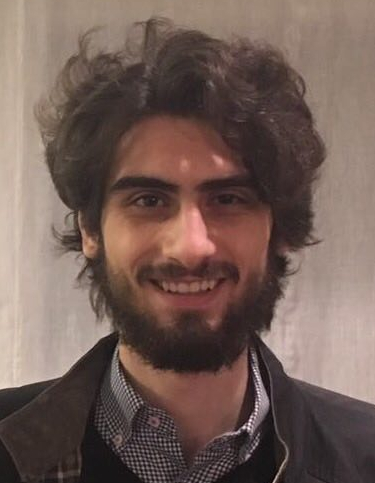
\includegraphics[width=0.13\textwidth]{images/hugo.jpg}}
    \end{flushleft}
\end{figure}

{\textsc {\Huge \vspace{5mm} \hspace{-13mm} Hugo Ferrando Seage}}\\

\begin{longtable}{rp{11cm}}
    EXPERIENCE
    & {\bf Student Internship at UEM} \hfill Sep 16 --- Mar 17\\
    & Prediction model of users and their opinion, based on Amazon review texts, using distributed computing\\
    \\
    & {\bf Talentum Startups --- Telefónica} \hfill Sep 16 --- Mar 17\\
    & Recommendation engine improvements of Telefonica's video on demand service \href{http://ver.movistarplus.es/}{Movistar+}\\
    \\
    & {\bf Student Internship at UEM} \hfill Aug 16 --- Sep 16\\
    & Motion detection of people swimming in pools and beaches using OpenCV\\
    \\
    & {\bf Web developer at Product Hackers} \hfill Jun 16 --- Oct 16\\
    & Creating web apps and chat bots using Angular 2 and Ionic 2 for mobile devices and the web\\
    \\
    & {\bf Student Internship at UEM} \hfill Sep 15 --- Jan 16\\
    & Android app to detect, alert and register traffic violations using OpenCV (computer vision and artificial intelligence)\\
    \\
    EDUCATION
    & {\bf Universidad Europea de Madrid} \hfill 2014 --- 2017\\
    & Bachelor's Degree in Computer Science\\
    \\
    & {\bf Universidad Politécnica de Madrid} \hfill 2012 --- 2014\\
    & Bachelor's Degree in Computer Science\\ 
    \\
    TECHNICAL KNOWLEDGE
    & {\bf Programming Languages}\\
    & Python, C/C++, Java, Bash, Javascript/NodeJS, Typescript\\
    \\
    & {\bf Frameworks}\\
    & Apache Spark, Angular 2, Ionic 2, Spring, NLTK, Bootstrap, jQuery\\
    \\
    & {\bf Tools}\\
    & Git, SSH, GPG, \LaTeX, Android SDK \& NDK, Nginx, Jenkins, OpenVPN, DNS (Knot, Unbound, BIND9, DNSSEC, DANE), Btrfs\\
    \\
    & {\bf Operating Systems}\\
    & GNU/Linux, Microsoft Windows, Android\\
    \\
    PROJECTS
    & \vspace{-8mm}
    \begin{itemize}[leftmargin=0cm,label={}]
        \item \href{https://github.com/hugo19941994/CHIP8-Emu}{CHIP-8 interpreter}: Executes CHIP-8 programs in Windows and Linux
        \item \href{https://github.com/hugo19941994/SpaceInvaders-Emu}{Intel 8080 emulator}: Executes Space Invaders in Windows
        \item {ovpn.io}: VPN provider using OpenVPN (offline)
        \item \href{https://github.com/hugo19941994/ViajeFacil}{ViajeFácil}: Management software for flight agencies. Colaboration between UEM \& Unisys
        \item \href{https://github.com/hugo19941994/CV-Parser}{CV-Parser}: CV management system using Name Entity Recognition and bayesian networks. Collaboration between UEM \& Everis
        \item \href{https://github.com/hugo19941994/robot}{Human Rescue Bot}: Laureate Awards for Excellence in Robotics Engineering 2016 1\textsuperscript{st} place winner
    \end{itemize}\\
    \\
    CERTIFICATIONS
    & \vspace{-8mm}
    \begin{itemize}[leftmargin=0cm,label={},noitemsep]
        \item Certificate in Advanced English (CAE)
        \item CCNA 1: Introduction to Networks
        \item CCNA 2: Routing and Switching Essentials
        \item CCNA 4: Connecting Networks
    \end{itemize}\\
    \\
    LANGUAGES
    & \vspace{-8mm}
    \begin{itemize}[leftmargin=0cm,label={},noitemsep]
        \item Advanced english
        \item Native spanish
        \item Native italian
        \item Basic french
    \end{itemize}
\end{longtable}
\end{document}
